\section{Introduction}
The reason why we choose capture the flag as our final project
is that, the game itself is fun and there are plenty of strategies
to win. In the following part, we'll briefly introduce the rule.

The map is divided into 2 halves: red(left) and blue(right). 
Each team with two agents must defend their own color territory while trying to eat food on the other side.
Red agents must defend food on red side and try to 
eat food on the blue side.  When on the red side, red agents are ghosts. When on the blue side,
red agents are Pacmans.

When a Pacman eats a food, the food is stored up inside the Pacman and removed
from the board.  When it returns to its own side, it deposits the food, earning 
1 point per food delivered.  If the Pacman is eaten before returning to its own side by a ghost, it loses all the food 
it is carrying and re-spawn to the start point as a ghost.  All the food become 
a cloud of food on the board.  No point rewards for eating Pacmans. 

Agent can only observe enemy 
agents’ position and direction if they are within 5 Manhattan distance from our agent. 
Otherwise, we will always get noisy distance reading. And this game is limited to 1200 
moves(300 moves for each agent), and the computation 
time for each agent is 1 second. 

The algorithm we are using is minimax algorithm with alpha-beta pruning. 
To deal with the noise in distance reading, we implemented particle filter, 
which is an established method for approximate inference of Hidden Markov Model. 
When test against two test agents baselineTeam and GoTeam, our agent won 19 games out of 20. 


\section{Approach}
Each team can control two agents. On our territory, they are in form of ghost (defensive agent), 
while on opponent's territory, they are in form of pacman (offensive agent). 
We have designed different strategies for the two types of agent.

\subsection{Development of offensive agent}
The goal of the offensive agent (pacman) is to return enemy's food safely. 
When making a choice for the next action, the offensive agent uses miniMax 
algorithm to choose actions that maximize the score. The score is calculated 
by evaluating a given game state with various heuristics. We have developed 
following strategies (heuristics) to guide the agent.

\subsubsection{Avoid enemy ghosts}
Although the first priority of our pacman is to return enemy's food, we want 
to do it in a safe way. Our pacman will try to avoid enemy ghosts by keeping 
distance to the nearest enemy. When enemy ghost is very close (maze distance <= 5) 
to our pacman, we choose to rush back to our side to dump the food we are carrying.

\subsubsection{Don't be too greedy}
If our pacman was caught by enemy ghosts, we will lose all food carried by 
that pacman. Thus we want our pacman to regularly return food to base and 
come back to eat more food. Currently we set a carrying-limit which equals 
to 6 at the beginning of the game, and this number decreases according to 
how much time is left in the game.

\subsubsection{Avoid obvious dead end}
There are many dead ends on the map. Our pacman should be able to 'see' an 
obvious dead end and avoid that, because run into a dead end will waste a 
step and increase the chance of being caught by the enemy. To help the pacman 
avoid dead end,  we scan the board at the very beginning of the game. For each 
legal position (not wall), we calculate its degree (how many directions can 
move when standing on that position) and store the result in a dictionary 
for later reference. When making a choice for the next move, our pacman should 
select a next position with a higher degree.


\begin{table}[!htb]
  \caption{Heuristics of offensive agent}
  \label{1}
  \begin{tabular}{ccl}
    \toprule
    Feature&Weight\\
    \midrule
    Board score & 1000\\
    Remaining food & -100\\
    Distance to closest food & -5\\
    Distance to enemy ghost & 20\\
    Distance to unseen ghost & 1\\
    Distance to scared ghost & -2\\
    Freedom to move & 1\\
  \bottomrule
\end{tabular}
\end{table}

\subsection{Development of defensive agent}
The goal of the defensive agent (ghost) is to defend our food. When making 
a choice for the next action, the defensive agent simply select an action 
from all legal actions that maximize the score. The score is calculated by 
evaluating a given gameState with various heuristics. We have developed 
following strategies (heuristics) to guide the agent.

\subsubsection{Chase enemy pacman}
Our ghost will keep monitoring invaders and try to send them back. For 
enemies that are insight, their exact location and direction are known, 
and our ghost will move towards the enemy to shorten the distance between 
them. For enemies that are unseen (only know a noise distance), we use 
particle filters to estimate their current location and move towards them.

\subsubsection{Follow potential enemies}
Our ghost should be able to follow potential enemies's move, and stop them 
from invading. To this end, we use particle filters to estimate enemy agents' 
location and make our ghost move according to the enemy's position.

\subsubsection{Stay close to frontline}
If there are no invaders, our ghost should stay close to frontline and patrol. 
This is more efficient than staying at rear.

\begin{table}[!htb]
  \caption{Heuristics of defensive agent}
  \label{2}
  \begin{tabular}{ccl}
    \toprule
    Feature&Weight\\
    \midrule
    Number of invaders insight & -1000\\
    Number of unseen invaders & -500\\
    Distance to invaders insight & -10\\
    Distance to unseen invaders & -5\\
    Distance to potential enemies & -2\\
    On Defense & 100\\
    Distance to frontline & 1\\
  \bottomrule
\end{tabular}
\end{table}

\subsection{Strategy of test agent GoTeam}
As our final team is one defensive agent and one offensive agent, we
implemented two offensive reflex, feature-based agents to test. 

To make the two agent collaborate, we divide the food on the map into two parts.
Each agent would approach the closest food in their own foodList.  Once they had consumed 
all the food in their foodList, they would return the food back to home and went after the 
food left on the map. 

To avoid the enemy ghost, we made the agent to retreat to middle line regardless of whether it
has eaten up its foodList to secure the food they have eaten.  Eat capsule first if it is close 
to the capsule or its teammate is close to the capsule.  This is also a way to collaborate.

Our test agent GoTeam is adventurous as to the distance to the opponent.  Although we can see 
the actual distance within 5 steps, we only make moves when the opponent is one step away from
us.  The advantage of it is the fact that we can eat as much food as possible. The disadvantage is somehow 
obvious, sometimes the agent will run into a dead end and caught by the enemies.

To determine the weight given to each of the above goals, we used the human thinking way.
Cause it is easy to rank the offensive agent's priority: 1. avoid ghost enemies, 2. eat
adjacent scared ghosts, 3. eat closest food. We set different feature and weight to reflect 
these priorities, as shown in Table 1.

\begin{table}[!htb]
  \caption{Heuristics of GoTeam agent}
  \label{3}
  \begin{tabular}{ccl}
    \toprule
    Feature&Weight\\
    \midrule
    successorScore & 100\\
    eatInvader & 5\\
    invaderOneStep & 1\\
    distanceToFood & -1\\
    distanceToShelter & 10\\
    eatCapsule & 10\\
    dangerousGhostOneStep & -20\\
    eatScaredGhostFirst & 1\\
    safeGhostOneStep & 0.1\\
    stopped & -10 \\
    eatFoodFirst & 1\\
  \bottomrule
\end{tabular}
\end{table}


\subsection{Locate unseen enemies}
One challenge in this game is that when enemy agents are far away (manhattan distance > 5), 
their exact positions are unknown. What we only know is a distance reading with noise up to .  
This is a classic hidden Markov Model (HMM), where we cannot make direct observations of the 
current state. To locate unseen enemies, we applied particle filters for approximate inference 
of the HMM \cite{CS188} \cite{Thrun02d} \cite{Wikipedia}. Briefly, we use a particle to represent 
a possible state (a legal location on the board). 
At time elapse step, we update the particle distribution according to enemy's moves. 
We expect the enemy agents will move towards our food, thus the moves that shorten the 
distance between enemy agent and our food will have a higher probability (we use 0.9). 
At observation step, we update the particle distribution according to current observation 
and normalize the probabilities. When the enemy agent is insight, we know its exact position. 
Otherwise we use the expected location which has the highest probability. Using this method, 
we were able to estimate enemy positions with high precision. This is critical to improve the 
efficiency of our defensive agent. In Figure 1, the depth of red color represents the approximate
locations of enemies. We can see that particle filter can almost locate every unseen enemies. 

\begin{figure}[!htb]
\includegraphics[height=1.7in, width=3.3in]{Picture.png}
\caption{Defensive agent with \texttt{Particle Filter}}
\end{figure}


\section{Results and Testing}
We did the test for our test agent GoTeam, and our final agent PacmanGo with/without particle filter
on default map.  Following are the results after running 20 games against each opponent team. 

\begin{table}[!htb]
  \caption{PacmanGo vs BaselineTeam result after 20 games}
  \label{4}
  \begin{tabular}{c|ccc}
    \toprule
    vs BaselineTeam & Win & Tie & Lose \\
    \midrule
    PacmanGo without Particle Filter & 85\% & 5\% & 10\%\\
    PacmanGo with Particle Filter & 95\% & 5\% & 0\%\\
    
  \bottomrule
\end{tabular}
\end{table}

\begin{table}[!htb]
  \caption{PacmanGo vs GoTeam result after 20 games}
  \label{5}
  \begin{tabular}{c|ccc}
    \toprule
    vs GoTeam & Win & Tie & Lose \\
    \midrule
    PacmanGo without Particle Filter & 70\% & 5\% & 25\%\\
    PacmanGo with Particle Filter & 95\% & 0\% & 5\%\\
    
  \bottomrule
\end{tabular}
\end{table}

From the test results we can see that the winning rate against GoTeam and BaselineTeam
improved after implementing the particle filter.

Then we used our final agent(with Particle Filter) against other teams.  Following are the results.

\begin{table}[!htb]
  \caption{PacmanGo vs Other teams result after 20 games}
  \label{6}
  \begin{tabular}{c|ccc}
    \toprule
    PacmanGo vs & Win & Tie & Lose \\
    \midrule
    Team1 & 0\% & 35\% & 65\%\\
    Team3 & 55\% & 10\% & 35\%\\
    Team4 & 0\% & 60\% & 40\%\\
    Team5 & 55\% & 0\% & 45\%\\
    
  \bottomrule
\end{tabular}
\end{table}

We have assessed the replay and observed several problems. 
One of them is deadlock between our offensive agent and opponent’s 
defensive agent(or our defensive agent and opponent’s offensive agent). 
These agents move back and forth near the border line, because the 
enemy ghost is in the way to the nearest food that our offensive 
agent wants to eat. This usually results in a tie game. 

Similarly, we utilized GoTeam to compete against other teams.

\begin{table}[!htb]
  \caption{GoTeam vs Other teams result after 20 games}
  \label{7}
  \begin{tabular}{c|ccc}
    \toprule
    GoTeam vs & Win & Tie & Lose \\
    \midrule
    Team1 & 30\% & 30\% & 40\%\\
    Team3 & 90\% & 0\% & 10\%\\
    Team4 & 70\% & 0\% & 30\%\\
    Team5 & 15\% & 0\% & 85\%\\
    
  \bottomrule
\end{tabular}
\end{table}

From the results, we noticed that the winning rate increases dramatically against Team 1, 
Team 3 and Team 4 comparing with PacmanGo's result. That's because GoTeam has better 
offense collaboration than PacmanGo. 

A common issue with PacmanGo and GoTeam is
fixed roles of agents. As a result, situations like these may occur in PacmanGo, after 
the offensive agent re-spawn at the start point and invaders observed in our side, the 
offensive agent will not assist the defensive agent so the enemy got away with food. 
Similarly, when there is no invaders, the defensive agent just stay and not attack, which
is conservative. On the contrary, GoTeam is way more adventurous, but it lacks defense 
action, once it is caught by enemy and re-spawn at home it will not defend only if the 
enemy is very close.

\section{Discussion}
There are still a lot of place that can be strengthened in our work.

To begin with, we considered the factor that the time and steps are limit, and fixed- 
role-agent cannot deal with all situations in a dynamic world, so our 
agent should change roles dynamically.  We could make agent switch between
different strategies, like Attack, Defense, Run, Chase, and let the agent
switch role between offense and defense based on how far the game has
progressed. Besides, when there is a deadlock, we could have made the agent 
switch plan or path. At last, our minimax depth is 1 so far. When the depth 
is 2, the execution time is too long. To solve the problem we may run the 
minimax in a simulate gameState to improve the depth to 2 or 3.

As to our test agent GoTeam, in some situations, it received better result than our final
agent because of its collaborative offense.  It can be improved also by changing 
strategy based on gameState, like when the board score is enough to win it can return
home to defend the territory, using the strategy of our final agent.

\begin{acks}
  We gratefully acknowledge John DeNero and Dan Klein in UC Berkeley 
  for developing the contest baseline code. 

  This work was performed by Chang, Weihan, and Yuan.

  Chang found the idea of the project. He implemented Minimax 
  and Particle Filter in our final agent. He
  wrote the approach of our final agent part. 
  Weihan arranged the code, meeting note, implemented agent test and 
  designed the heuristics of final agent. 
  He wrote the introduction, test and result part in this paper.
  Yuan implemented test agent GoTeam, organize the team meetings and 
  took charge of the presentation PPT. He wrote the rest part of the 
  paper and combine the paper using latex.

  We want to express our gratitude to Prof.Stacy, what he taught in
  class not only gives us inspiration, but also is very useful in our 
  future study and work. Also, we would like to thank our TA Dan and Navya,
  who have been assisting us in solving problems during the course.  And special
  thanks to Pedro, Nutchanon, Dan, Sophie for giving us wonderful lectures.

\end{acks}

\begin{comment}

\subsection{Type Changes and {\itshape Special} Characters}

We have already seen several typeface changes in this sample.  You can
indicate italicized words or phrases in your text with the command
\texttt{{\char'134}textit}; emboldening with the command
\texttt{{\char'134}textbf} and typewriter-style (for instance, for
computer code) with \texttt{{\char'134}texttt}.  But remember, you do
not have to indicate typestyle changes when such changes are part of
the \textit{structural} elements of your article; for instance, the
heading of this subsection will be in a sans serif\footnote{Another
  footnote here.  Let's make this a rather long one to see how it
  looks.} typeface, but that is handled by the document class file.
Take care with the use of\footnote{Another footnote.}  the
curly braces in typeface changes; they mark the beginning and end of
the text that is to be in the different typeface.

You can use whatever symbols, accented characters, or non-English
characters you need anywhere in your document; you can find a complete
list of what is available in the \textit{\LaTeX\ User's Guide}
\cite{Lamport:LaTeX}.

\subsection{Math Equations}
You may want to display math equations in three distinct styles:
inline, numbered or non-numbered display.  Each of
the three are discussed in the next sections.

\subsubsection{Inline (In-text) Equations}
A formula that appears in the running text is called an
inline or in-text formula.  It is produced by the
\textbf{math} environment, which can be
invoked with the usual \texttt{{\char'134}begin\,\ldots{\char'134}end}
construction or with the short form \texttt{\$\,\ldots\$}. You
can use any of the symbols and structures,
from $\alpha$ to $\omega$, available in
\LaTeX~\cite{Lamport:LaTeX}; this section will simply show a
few examples of in-text equations in context. Notice how
this equation:
\begin{math}
  \lim_{n\rightarrow \infty}x=0
\end{math},
set here in in-line math style, looks slightly different when
set in display style.  (See next section).

\subsubsection{Display Equations}
A numbered display equation---one set off by vertical space from the
text and centered horizontally---is produced by the \textbf{equation}
environment. An unnumbered display equation is produced by the
\textbf{displaymath} environment.

Again, in either environment, you can use any of the symbols
and structures available in \LaTeX\@; this section will just
give a couple of examples of display equations in context.
First, consider the equation, shown as an inline equation above:
\begin{equation}
  \lim_{n\rightarrow \infty}x=0
\end{equation}
Notice how it is formatted somewhat differently in
the \textbf{displaymath}
environment.  Now, we'll enter an unnumbered equation:
\begin{displaymath}
  \sum_{i=0}^{\infty} x + 1
\end{displaymath}
and follow it with another numbered equation:
\begin{equation}
  \sum_{i=0}^{\infty}x_i=\int_{0}^{\pi+2} f
\end{equation}
just to demonstrate \LaTeX's able handling of numbering.

\subsection{Citations}
Citations to articles~\cite{bowman:reasoning,
clark:pct, braams:babel, herlihy:methodology},
conference proceedings~\cite{clark:pct} or maybe
books \cite{Lamport:LaTeX, salas:calculus} listed
in the Bibliography section of your
article will occur throughout the text of your article.
You should use BibTeX to automatically produce this bibliography;
you simply need to insert one of several citation commands with
a key of the item cited in the proper location in
the \texttt{.tex} file~\cite{Lamport:LaTeX}.
The key is a short reference you invent to uniquely
identify each work; in this sample document, the key is
the first author's surname and a
word from the title.  This identifying key is included
with each item in the \texttt{.bib} file for your article.

The details of the construction of the \texttt{.bib} file
are beyond the scope of this sample document, but more
information can be found in the \textit{Author's Guide},
and exhaustive details in the \textit{\LaTeX\ User's
Guide} by Lamport~\shortcite{Lamport:LaTeX}.

This article shows only the plainest form
of the citation command, using \texttt{{\char'134}cite}.

Some examples.  A paginated journal article \cite{Abril07}, an enumerated
journal article \cite{Cohen07}, a reference to an entire issue \cite{JCohen96},
a monograph (whole book) \cite{Kosiur01}, a monograph/whole book in a series (see 2a in spec. document)
\cite{Harel79}, a divisible-book such as an anthology or compilation \cite{Editor00}
followed by the same example, however we only output the series if the volume number is given
\cite{Editor00a} (so Editor00a's series should NOT be present since it has no vol. no.),
a chapter in a divisible book \cite{Spector90}, a chapter in a divisible book
in a series \cite{Douglass98}, a multi-volume work as book \cite{Knuth97},
an article in a proceedings (of a conference, symposium, workshop for example)
(paginated proceedings article) \cite{Andler79}, a proceedings article
with all possible elements \cite{Smith10}, an example of an enumerated
proceedings article \cite{VanGundy07},
an informally published work \cite{Harel78}, a doctoral dissertation \cite{Clarkson85},
a master's thesis: \cite{anisi03}, an online document / world wide web
resource \cite{Thrun02d}, a video game (Case 1) \cite{Wikipedia} and (Case 2) \cite{CS188}



\subsection{Tables}
Because tables cannot be split across pages, the best
placement for them is typically the top of the page
nearest their initial cite.  To
ensure this proper ``floating'' placement of tables, use the
environment \textbf{table} to enclose the table's contents and
the table caption.  The contents of the table itself must go
in the \textbf{tabular} environment, to
be aligned properly in rows and columns, with the desired
horizontal and vertical rules.  Again, detailed instructions
on \textbf{tabular} material
are found in the \textit{\LaTeX\ User's Guide}.

Immediately following this sentence is the point at which
Table~\ref{tab:freq} is included in the input file; compare the
placement of the table here with the table in the printed
output of this document.

\begin{table}
  \caption{Frequency of Special Characters}
  \label{tab:freq}
  \begin{tabular}{ccl}
    \toprule
    Non-English or Math&Frequency&Comments\\
    \midrule
    \O & 1 in 1,000& For Swedish names\\
    $\pi$ & 1 in 5& Common in math\\
    \$ & 4 in 5 & Used in business\\
    $\Psi^2_1$ & 1 in 40,000& Unexplained usage\\
  \bottomrule
\end{tabular}
\end{table}

To set a wider table, which takes up the whole width of the page's
live area, use the environment \textbf{table*} to enclose the table's
contents and the table caption.  As with a single-column table, this
wide table will ``float'' to a location deemed more desirable.
Immediately following this sentence is the point at which
Table~\ref{tab:commands} is included in the input file; again, it is
instructive to compare the placement of the table here with the table
in the printed output of this document.


\begin{table*}
  \caption{Some Typical Commands}
  \label{tab:commands}
  \begin{tabular}{ccl}
    \toprule
    Command &A Number & Comments\\
    \midrule
    \texttt{{\char'134}author} & 100& Author \\
    \texttt{{\char'134}table}& 300 & For tables\\
    \texttt{{\char'134}table*}& 400& For wider tables\\
    \bottomrule
  \end{tabular}
\end{table*}
% end the environment with {table*}, NOTE not {table}!



\subsection{Figures}

Like tables, figures cannot be split across pages; the best placement
for them is typically the top or the bottom of the page nearest their
initial cite.  To ensure this proper ``floating'' placement of
figures, use the environment \textbf{figure} to enclose the figure and
its caption.

This sample document contains examples of \texttt{.eps} files to be
displayable with \LaTeX.  If you work with pdf\LaTeX, use files in the
\texttt{.pdf} format.  Note that most modern \TeX\ systems will convert
\texttt{.eps} to \texttt{.pdf} for you on the fly.  More details on
each of these are found in the \textit{Author's Guide}.

\begin{figure}
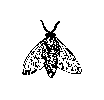
\includegraphics{fly}
\caption{A sample black and white graphic.}
\end{figure}

\begin{figure}
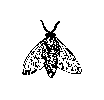
\includegraphics[height=1in, width=1in]{fly}
\caption{A sample black and white graphic
that has been resized with the \texttt{includegraphics} command.}
\end{figure}




\begin{figure*}
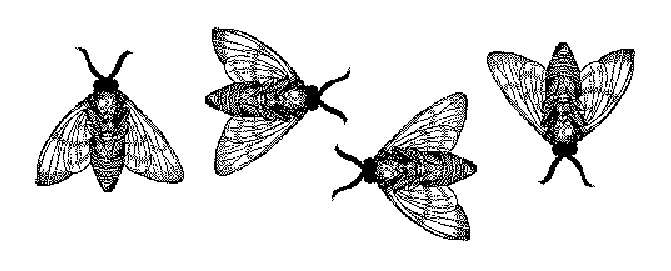
\includegraphics{flies}
\caption{A sample black and white graphic
that needs to span two columns of text.}
\end{figure*}


\begin{figure}
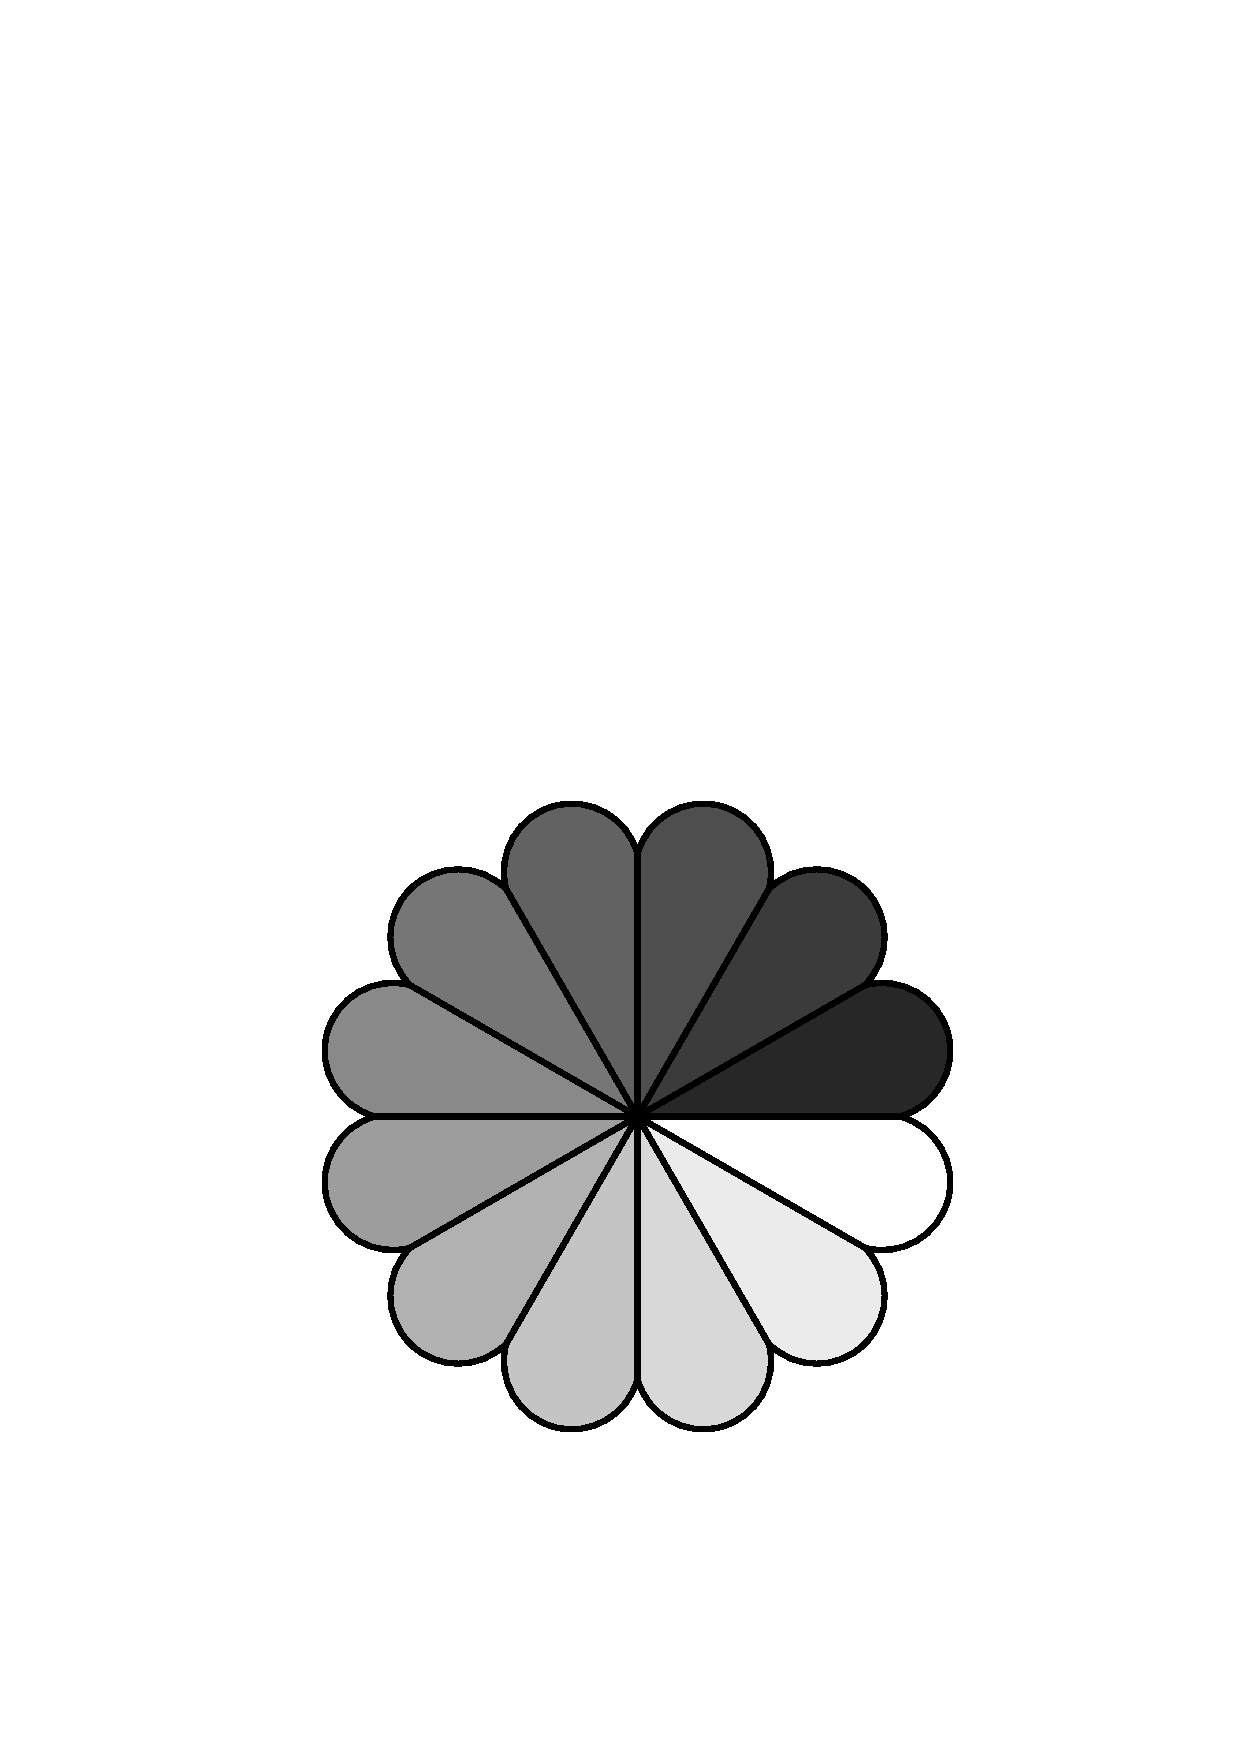
\includegraphics[height=1in, width=1in]{rosette}
\caption{A sample black and white graphic that has
been resized with the \texttt{includegraphics} command.}
\end{figure}


%\end{document}  % This is where a 'short' article might terminate



\appendix
%Appendix A
\section{Headings in Appendices}
The rules about hierarchical headings discussed above for
the body of the article are different in the appendices.
In the \textbf{appendix} environment, the command
\textbf{section} is used to
indicate the start of each Appendix, with alphabetic order
designation (i.e., the first is A, the second B, etc.) and
a title (if you include one).  So, if you need
hierarchical structure
\textit{within} an Appendix, start with \textbf{subsection} as the
highest level. Here is an outline of the body of this
document in Appendix-appropriate form:
\subsection{Introduction}
\subsection{The Body of the Paper}
\subsubsection{Type Changes and  Special Characters}
\subsubsection{Math Equations}
\paragraph{Inline (In-text) Equations}
\paragraph{Display Equations}
\subsubsection{Citations}
\subsubsection{Tables}
\subsubsection{Figures}
\subsubsection{Theorem-like Constructs}
\subsubsection*{A Caveat for the \TeX\ Expert}
\subsection{Conclusions}
\subsection{References}
Generated by bibtex from your \texttt{.bib} file.  Run latex,
then bibtex, then latex twice (to resolve references)
to create the \texttt{.bbl} file.  Insert that \texttt{.bbl}
file into the \texttt{.tex} source file and comment out
the command \texttt{{\char'134}thebibliography}.
% This next section command marks the start of
% Appendix B, and does not continue the present hierarchy
\section{More Help for the Hardy}

Of course, reading the source code is always useful.  The file
\path{acmart.pdf} contains both the user guide and the commented
code.
\end{comment}

